\section{Results - Extended model}

\textbf{HUSK AT ÆNDRE Y AKSEN FRA AGE TIL PARTICPATION RATE OF HOURS! PLUS ÆNDRE X-AKSEN TIL age}

\begin{itemize}
    \item Gennemsnit antal arbejdede timer
    \item Procentdel af kvinder i arbejdsstyrken
    \item Event Grafer (fortæl også om hvorfor man ikke kan kopiere Kleven 1:1. -> mænds arbejds udbud er ikke endogent!
    \begin{itemize}
        \item Løn
        \item arbejds tid
        \item Participation rate
        \item Earnings
    \end{itemize}
\end{itemize}

To envestigate the results I simulate 200.000 households using the optimal $\beta_L = 24.49$. Using this sample i can do counter factual analysis of households that do get children, and households that do not get children. Figure \ref{fig:ext_model_working_hours} show the average number of working hours of the simulations compared to the true number of hours worked by women. This extended model fits the data considerably better than the simple model, as shown by figure \ref{fig:dqi_model1_average_path_sim_vs_empirical}. Again the models also differ in the action space, where this extended model do not allow for working more than 37 hours a week - the old model did. The average number of hours worked hours is calculated by conditioning on the supplied number of hours working must be above 0. The figure also shows the average number of hours supplied by women when they get children at their specific age. This is true for age 25, 30 and age 35. These households get one child and only one child. For these house holds i do not condition on wether $H>0$. Looking to these households very steep dips in the supplied number of hours are very obvious, at about 5 hours for each of the three age groups. The cohorts of households that get a child at age 30 and 35 year dip to a permanently lower number of supplied hours, where as the cohort that get a child at age 25, get an initial dip, but do at after a certain period of time readjust the number of supplied hours. For all three cohorts the initial dip when the housholds get the child is about 5 hours.

\begin{figure}
    \centering
    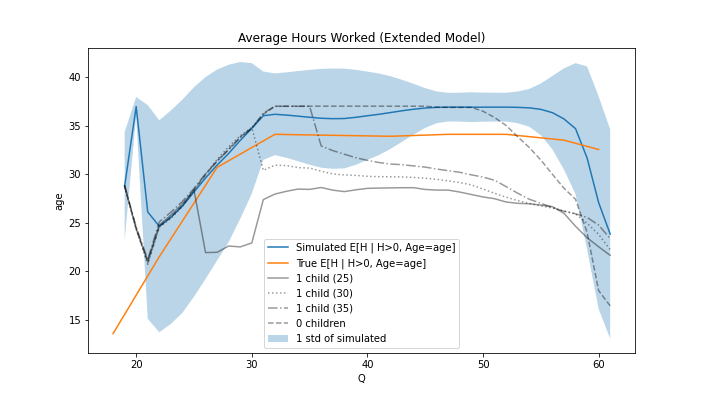
\includegraphics[scale=0.4]{figures/extended_model_average_hours.png}
    \caption{Extended Model Working Hours - Empirical Vs. Simulated}
    \label{fig:ext_model_working_hours}
\end{figure}

Figure \ref{fig:ext_model_particpation_rates} shows the participation rate over the life cycle. The average participation of all simulations is $81.7 \%$ letting the overall number of women out of the workforce be equal to $18.3$ comparing to the the number used for the optimization of $\beta_L$ which was $15 \%$, must be considered a good fit. I have not found good data from Statistics Denmark showing women's average participation rate over the life cycle, implying it's hard for to make inference over the participation rate over the life cycle. However a couple of things can be noted. First and foremost the simulations show a downward sloping trend of participation rates over the life cycle. XXX Grimm Bonneuil 2001 have investigated female labour participation rate in France over the life cycle. Their data suggest that picture is not totally unrealistic. Certain things should however be noted. Their sample ends in 1998, and looking to that data, the downward sloping trend do seem to be less clear. 

\begin{figure}
    \centering
    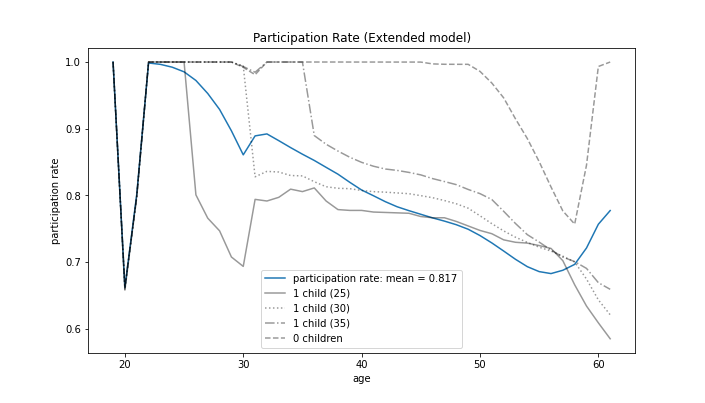
\includegraphics[scale=0.4]{figures/extended_model_participation_rates.png}
    \caption{Participation rates}
    \label{fig:ext_model_particpation_rates}
\end{figure}


\begin{figure}[ht]
\begin{subfigure}{.5\textwidth}
  \centering
  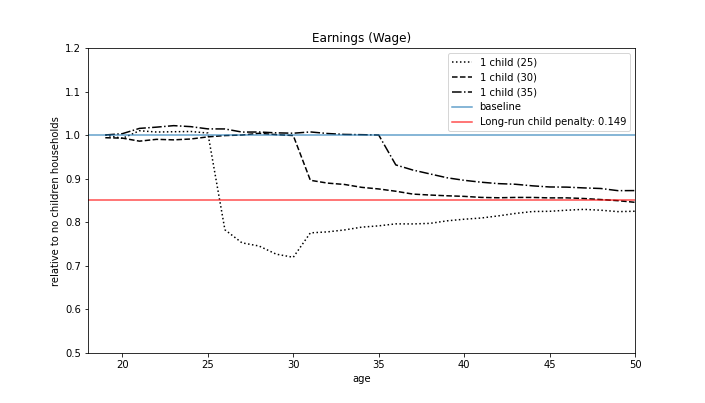
\includegraphics[width=1\linewidth]{figures/extended_model_event_earnings.png}
  \caption{Earnings}
  \label{fig:ext_model_event_earnings}
\end{subfigure}%
\begin{subfigure}{.5\textwidth}
  \centering
  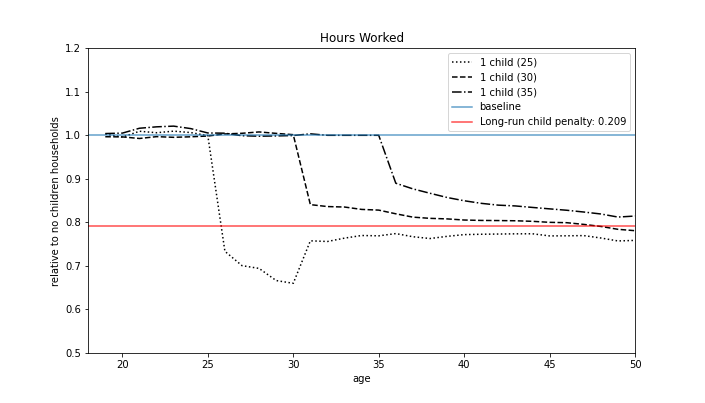
\includegraphics[width=1\linewidth]{figures/extended_model_event_hours_worked.png}
  \caption{Hours Worked}
  \label{fig:ext_model_event_hours}
\end{subfigure}
    \caption{Impact of Children (Earnings and Worked Hours)}
    \label{fig:ext_model_impact_earnings_hours}
\end{figure}



\begin{figure}[ht]
\begin{subfigure}{.5\textwidth}
  \centering
  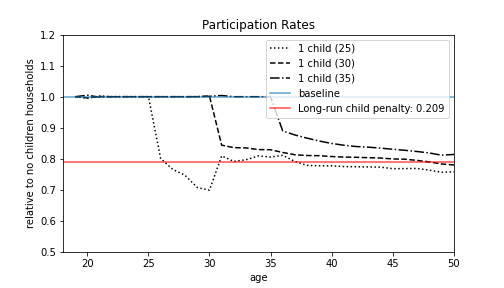
\includegraphics[width=1\linewidth]{figures/extended_model_event_participation_rates.png}
  \caption{Participation Rates}
  \label{fig:ext_model_event_partipation}
\end{subfigure}%
\begin{subfigure}{.5\textwidth}
  \centering
  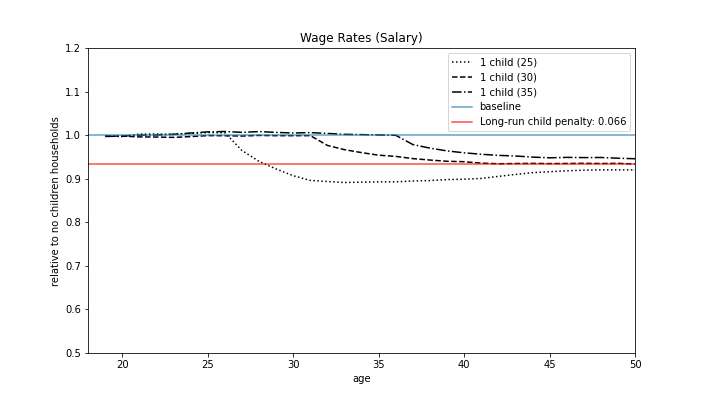
\includegraphics[width=1\linewidth]{figures/extended_model_event_wage_rates.png}
  \caption{Wage Rates}
  \label{fig:ext_model_event_wage_rates}
\end{subfigure}
    \caption{Impact of Children (Participation Rates and Wage Rates)}
    \label{fig:ext_model_impact_participation_wage}
\end{figure}

ALTERNATIVE FIGURER -> MATCHENDE Kleven

\begin{figure}[ht]
\begin{subfigure}{.5\textwidth}
  \centering
  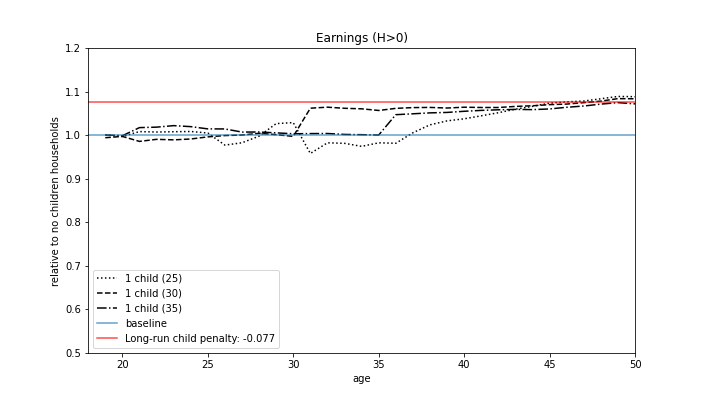
\includegraphics[width=1\linewidth]{figures/extended_model_event_earnings_H>0.png}
  \caption{Earnings Conditional on $H > 0$}
  \label{fig:ext_model_event_earnings_alt}
\end{subfigure}%
\begin{subfigure}{.5\textwidth}
  \centering
  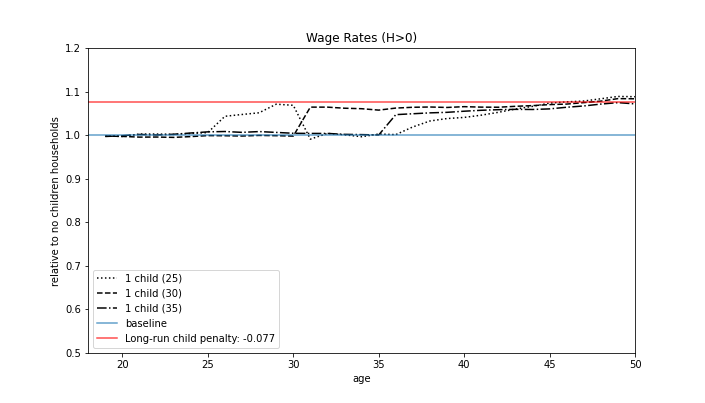
\includegraphics[width=1\linewidth]{figures/extended_model_event_wage_rates_H>0.png}
  \caption{Wage Rates Conditional on $H>0$}
  \label{fig:ext_model_event_wage_rates_alt}
\end{subfigure}
    \caption{Impact of Children conditional on $H>0$}
    \label{fig:ext_model_impact_alt}
\end{figure}


\begin{table}[ht]
    \centering
    \begin{tabular}{lrrr}
\toprule
                     &  Kleven et al. &  result &  result (H > 0) \\
\midrule
            Earnings &          0.194 &   0.149 &          -0.077 \\
        Hours worked &          0.097 &   0.209 &           0.000 \\
 Participation rates &          0.130 &   0.209 &             NaN \\
          Wage rates &          0.194 &   0.066 &          -0.077 \\
\bottomrule
\end{tabular}

    \caption{Long run penalties comparison}
    \label{tab:extended_results}
\end{table}




